\question (哈尔滨工程大学,2003年)( )存储结构对程序员是透明的
\par\twoch{通用寄存器}{主存}{\textcolor{red}{控制寄存器}}{堆栈}
\begin{solution}C。
通用寄存器、主存、堆栈都是可以被程序员编程操作的,而控制寄存器是控制器的内部结构,只关乎计算机系统的设计人员,对程序员是透明的。
\end{solution}
\question 主存储器主要性能指标有 I.存储周期 II.存储容量 III.存取时间
IV.存储器带宽
\par\twoch{I、II}{I、II和IV}{I、III和IV}{\textcolor{red}{全部都是}}
\begin{solution}D。 主存的主要技术指标包括:
存储容量,指某计算机实际配置的容量,通常来说,它小于最大可配置容量(主存地址空间大小)。
存取时间,指执行一次读操作或写操作的时间,分读出时间和写入时间两种。
存储周期,指存储器进行连续两次独立的读或写操作所需要的最小时间间隔,它通常大于存取时间。
存储器带宽,指单位时间内从存储器读出或写入存储器的最大信息量。
\end{solution}
\question 下列关于主存的描述中,正确的是
\par\fourch{CPU访存时间由主存容量决定}{ROM和RAM在主存中是单独编址的}{\textcolor{red}{ROM中任一单元可随机访问}}{DRAM中是破坏性读出,因此需要读后重写}
\begin{solution}C。
由于主存是随机存取的,CPU访存时间与主存容量无关。通常主存由ROM和RAM构成,它们是统一编址的。只有单管的DRAM是破坏性读出,而多管的DRAM是非破坏性读出。ROM的内容只能随机地读出而不能写入。
\end{solution}
\question (重庆大学,2000年)下列叙述正确的是
\par\twoch{\textcolor{red}{主存可由RAM和ROM组成}}{主存只能由ROM组成}{主存只能由RAM组成}{主存只能由SRAM组成}
\begin{solution}A。
主存一般由ROM和RAM组成,并且在RAM中使用DRAM来制作主存。SRAM一般用来制作Cache。
\end{solution}
\question (重庆大学)下列关于存储器的描述,正确的是
\par\fourch{CPU访存时间由存储器容量决定}{\textcolor{red}{ROM和RAM在存储器中采用统一编址}}{ROM中任意一个单元可以随机读和写}{DRAM是破坏性读出,因此需要读后重写}
\begin{solution}B。
CPU访问的时间和存储器的容量没有关系,故A选项错误;主存的空间由RAM和ROM组成,而且统一编址,故B选项正确;ROM是一种特殊的RAM,存储器只能读出不能写入,故C选项错误;单管的DRAM是破坏性读出,但是多管的DRAM是非破坏性读出,故D选项错误。
\end{solution}
\question 下述说法中正确的是 Ⅰ.半导体RAM信息可读可写,且断电后仍能保持记忆
Ⅱ.动态RAM是易失性RAM,而静态RAM中的存储信息是不易失的
Ⅲ.半导体RAM是易失性RAM,但只要电源不断电,所存信息是不丢失的
Ⅳ.半导体RAM是非易失性的RAM
\par\twoch{Ⅰ、Ⅱ}{只有Ⅲ}{Ⅱ、Ⅳ}{\textcolor{red}{全错}}
\begin{solution}D。
半导体RAM,无论静态RAM还是动态RAM都是易失性的,断电后信息都将丢失。RAM是可读可写,而ROM只读。对于Ⅲ来讲,DRAM即使不断电,如果在规定的时间内没有及时刷新,则信息也会消失。
归纳总结:易失性存储器,即断电后存储信息消失的存储器;断电后信息仍然保存的存储器被称为非易失性存储器。显然半导体RAM是易失性的存储器。
\end{solution}
\question 若数据在存储器中采用以低字节地址为字地址的存放方式(小端存储),则十六进制数12345678H按自己地址由小到大依次存为
\par\twoch{12345678}{87654321}{\textcolor{red}{78563412}}{34127856}
\begin{solution}其实大端法、小端法就是字节在内存中的存放顺序问题,如果某数据只有一个字节,也就不存在什么大端法和小端法了。
概念:
小端法就是低位字节排放在内存的低地址端,高位字节排放在内存的高地址端。
大端法就是高位字节排放在内存的低地址端,低位字节排放在内存的高地址端。
举例说明:16bit宽的数0x1234(左边是高字节,右边是低字节),在小端法模式下,CPU内存中的存放方式(假设从地址0x4000开始存放)如下。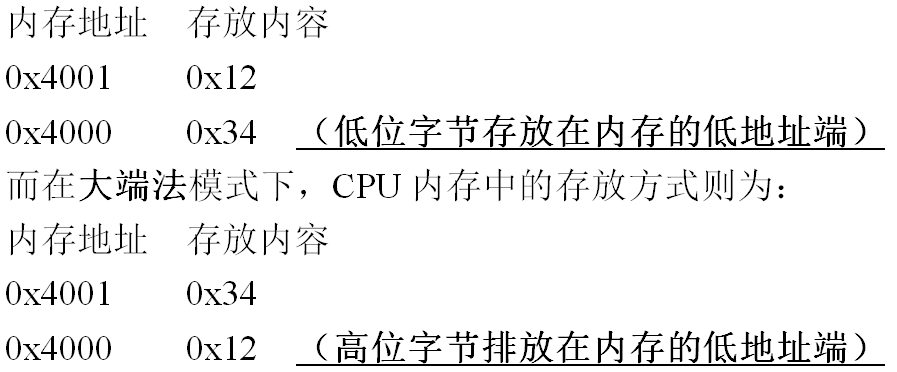
\includegraphics[width=2.31250in,height=0.95833in]{computerassets/EF77748026784D6F780F5F685958E7B8.png}
\end{solution}
\question 某容量为256MB的存储器由若干4M*8位DRAM芯片构成,该DRAM芯片的地址引脚和数据引脚总数是(
)
\par\twoch{\textcolor{red}{19}}{22}{30}{36}
\begin{solution}本题考察DRAM半导体存储芯片的结构,很多不熟悉DRAM工作原理的考生很有可能得出22+8=30的结论。因为4M的地址空间需要22根地址线来标识,加上8根数据线。其实这是不对的,考生在平时可能很少接触到关于DRAM的引脚复用的知识点。我们知道半导体存储芯片的译码驱动方式有线选法和重合法,动态RAM是由许多基本存储元按照行和列地址引脚复用来组成的。我们要选中一个单元就需要行地址(11位)加上列地址(11位),现在采用引脚复用,只需11位,但需要两次发送地址(行地址和列地址)。故11+8=19。
【总结】关于DRAM的引脚复用还是第一次考到,考生记住此知识点即可。另外,此题存在迷惑性,很多考生稍不注意就以为考察的是存储器的扩充,导致误选,题目中问的是DRAM芯片的引脚,因此与存储器无关。
\end{solution}
